\chapter{Spectral uncertainty and exact completion}\label{ch:spectrum}
\chapterlead{A useful operator approximation is not automatically a useful tail
approximation. This chapter transports phase-pruning error to eigenvalue
intervals, measures unresolved range through trace information, and completes
small residual ranges exactly. A separate post-verification theorem connects
stored binary64 factors to rigorous spectral intervals.}
\section{From phase pruning to certified quadratic-form tails}\label{sec:final-22}

The previous sections certify the effect of phase pruning on Krylov
propagation.  A SKAT-like test ultimately depends on the spectrum itself, so
one more bridge is needed:
\[
\text{phase pruning}
\longrightarrow
\text{operator error}
\longrightarrow
\text{spectral error}
\longrightarrow
\text{tail-probability error}.
\]

\subsection{Block-norm operator domination}

Let
\[
E=H-H_0
\]
be the self-adjoint error introduced by phase pruning.  Using the same
orthogonal phase projectors \(P_h\), define
\[
\mathcal C_{hg}
=
\|P_hEP_g\|_2.
\]

\begin{theorem}[Block-norm operator certificate]\label{claim:final-22-1}
\[
\boxed{
\|E\|_2
\le
\|\mathcal C\|_2.
}
\]
\end{theorem}

\begin{proof}
For any vector \(x\), let
\[
r_g=\|P_gx\|_2.
\]
Then
\[
\|P_hEx\|_2
\le
\sum_g
\|P_hEP_g\|_2\,\|P_gx\|_2
=
(\mathcal C r)_h.
\]
Orthogonality of the phase decomposition gives
\[
\|Ex\|_2^2
=
\sum_h\|P_hEx\|_2^2
\le
\|\mathcal C r\|_2^2
\le
\|\mathcal C\|_2^2\|r\|_2^2
=
\|\mathcal C\|_2^2\|x\|_2^2.
\]
Taking the supremum over unit vectors proves the claim.
\end{proof}

The important computational point is that \(\mathcal C\) is only a
phase-by-phase matrix.  The same block norms already used to construct the
polyphase scheduler therefore provide a global operator certificate.

\subsection{Weyl enclosure of the quadratic-form coefficients}

Assume
\[
H\succeq0
\]
and let the eigenvalues of \(H\) and \(H_0\), in decreasing order, be
\[
\lambda_i
\qquad\text{and}\qquad
\mu_i.
\]
If
\[
\|H-H_0\|_2\le\varepsilon,
\]
Weyl's inequality gives
\[
|\lambda_i-\mu_i|\le\varepsilon.
\]

\begin{corollary}[Positive spectral interval]\label{claim:final-22-2}
For every \(i\),
\[
\boxed{
\ell_i
=
\max\{0,\mu_i-\varepsilon\}
\le
\lambda_i
\le
u_i
=
\max\{0,\mu_i+\varepsilon\}.
}
\]
\end{corollary}

This remains valid even if symmetric phase pruning makes \(H_0\) slightly
indefinite.

\subsection{Certified generalized-\texorpdfstring{\(\chi^2\)}{chi-square} tail bracket}

For independent standard normal variables \(Z_i\), define
\[
Q_-=\sum_i\ell_iZ_i^2,
\qquad
Q=\sum_i\lambda_iZ_i^2,
\qquad
Q_+=\sum_i u_iZ_i^2.
\]

\begin{theorem}[Stochastic tail enclosure]\label{claim:final-22-3}
For every threshold \(q\),
\[
\boxed{
\Pr(Q_-\ge q)
\le
\Pr(Q\ge q)
\le
\Pr(Q_+\ge q).
}
\]
\end{theorem}

\begin{proof}
Couple all three quadratic forms using the same normal variables \(Z_i\).
Since
\[
0\le\ell_i\le\lambda_i\le u_i
\]
for every \(i\),
\[
Q_-\le Q\le Q_+
\]
almost surely.  Taking upper-tail events yields the result.
\end{proof}

The endpoint probabilities are separate tail queries. Each must satisfy the
hypotheses of the numerical backend used to evaluate it. In particular, zero
lower coefficients can reduce the active rank below the directed backend's
coverage. The stochastic enclosure remains valid in that case, but it does
not by itself supply a supported numerical evaluation. Numerical error is
separate from the spectral uncertainty above.

\subsection{A dual-budget pruning rule}

The local Krylov certificate from the previous section and the global spectral
certificate answer different questions.  The former asks whether omitted
couplings matter to the current Krylov query. The latter asks whether they can
move the spectrum enough to matter to the final test.

An execution schedule should therefore enforce
\[
\boxed{
\sum_{e\in\mathcal O}\beta_e^{(k)}
\le
\tau_K,
\qquad
\|\mathcal C_{\mathcal O}\|_2
\le
\tau_\lambda.
}
\]

The implementation uses a conservative greedy rule: phase pairs are considered
in increasing query-risk order, and a pair is omitted only when adding it
preserves both inequalities.  The rule is certified but is not claimed to be
globally optimal under the two simultaneous constraints.

\begin{figure}[htbp]
\centering
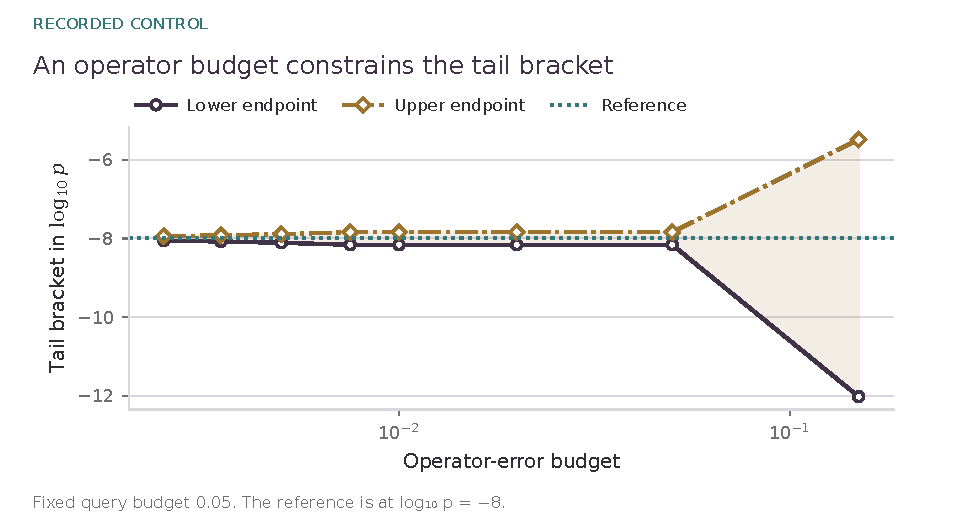
\includegraphics[width=\linewidth]{figures_production/figure_14_dual_budget_tail_bridge.pdf}
\caption{Tail brackets under a fixed query budget and varying operator budgets. The dotted reference is at $\log_{10}p=-8$. A sufficiently loose operator budget admits a strong coupling and widens the bracket even though the query-local constraint still passes.}
\label{fig:dual-budget-tail}
\end{figure}

In the deterministic ten-phase experiment, fixing the query budget at
\(0.05\) and the operator budget at \(0.005\) removed \(23\) of \(45\)
undirected phase pairs.  At a reference probability near \(10^{-8}\), the analytic
tail bracket was
\[
10^{-8.11143}
\le
p
\le
10^{-7.89036},
\]
a width of about \(0.221\) decades. These endpoints summarize the
real-arithmetic error analysis evaluated in floating point, not a directed
rounding enclosure. With an operator budget of \(0.0075\),
\(34\) pairs were removed and the interval widened to about \(0.320\)
decades.  By contrast, allowing a strong coupling to be removed under a very
loose operator budget produced a multi-decade interval.

\subsection{Certify after prune}

There is a second route that does not use the pruned operator as the final
spectral approximation.  Let \(U\) be any orthonormal sample-space basis,
possibly generated cheaply from a pruned or approximate Krylov process, and
define
\[
B=U^\top A,
\qquad
F=(I-UU^\top)A,
\qquad
\delta=\|F\|_2.
\]

\begin{theorem}[Range-core singular-value certificate]\label{claim:final-22-4}
For $A\in\mathbb R^{n\times m}$, list the singular values of $A$ and
$B$ in decreasing order and pad both lists with zeros to length $n$.
Write these lists as $\sigma_i(A)$ and $\widetilde\sigma_i(B)$,
respectively. They are the square roots of the $n$ eigenvalues of
$AA^\top$ and $(UB)(UB)^\top$. Then, for $1\le i\le n$,
\[
\boxed{
\left|
\sigma_i(A)
-
\widetilde\sigma_i(B)
\right|
\le
\delta.
}
\]
Consequently,
\[
\max\{0,\widetilde\sigma_i(B)-\delta\}^2
\le
\lambda_i(AA^\top)
\le
\left(
\widetilde\sigma_i(B)+\delta
\right)^2.
\]
\end{theorem}

\begin{proof}
Because \(U\) has orthonormal columns,
\[
A=UB+F
\]
and
\[
\|A-UB\|_2=\|F\|_2=\delta.
\]
The nonzero singular values of $UB$ and $B$ agree, with multiplicity,
and their zero-padded lists agree in the stated ambient convention.
The standard singular-value perturbation inequality gives the stated bound.
Squaring the nonnegative endpoints gives the eigenvalue interval.
\end{proof}

This provides a useful architecture:
\[
\boxed{
\begin{gathered}
\text{pruned operator for basis discovery}\\
\longrightarrow\ \text{exact streamed factor check}\\
\longrightarrow\ \text{certified spectral core}
\end{gathered}
}
\]

\subsection{A retained negative result}

The preceding theorem is exact, but a correct interval need not be useful.

In a full-rank \(50\times50\) stress test, a pruned Krylov basis of dimensions
\(12\) through \(48\) left range residuals between roughly \(0.87\) and
\(0.99\) times the leading singular value.  The corresponding \(10^{-8}\)
tail intervals were therefore vacuous or thousands of decades wide.  At
dimension \(50\), the range residual fell to approximately
\(1.2\times10^{-15}\), and the tail interval collapsed to the exact value.

\begin{figure}[htbp]
\centering
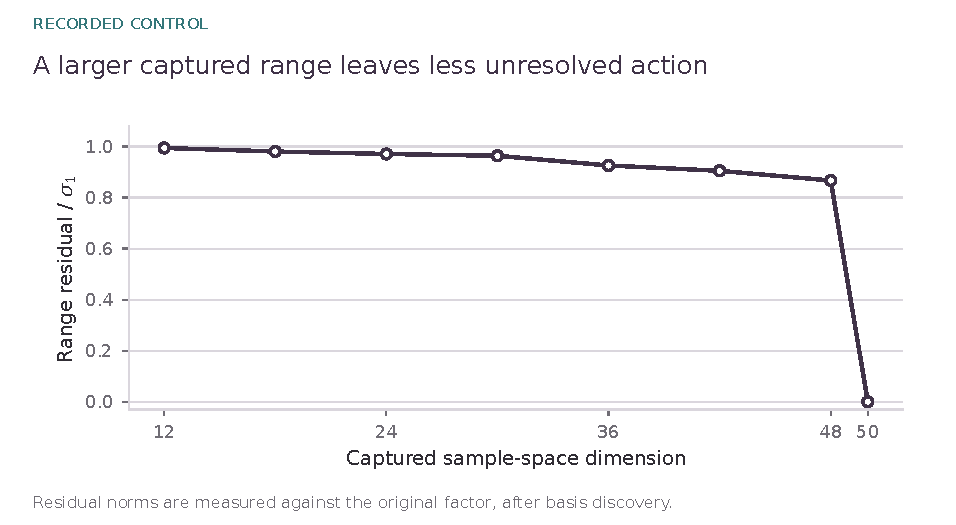
\includegraphics[width=\linewidth]{figures_production/figure_15_range_core_certification.pdf}
\caption{Range residual measured against the original factor after basis discovery. Increasing captured dimension reduces unresolved action in this control, but a useful deep-tail bracket still requires a sufficiently small residual. Basis discovery and certification remain separate steps.}
\label{fig:range-core-cert}
\end{figure}

The practical lesson is that range-core certification is a stopping test, not
a promise that a severely incomplete basis automatically yields a useful
full-spectrum tail bound.



\section{Trace-aware residual certification and exact completion}\label{sec:final-23}

The spectral bridge in the preceding section used an operator-norm residual as
if every unresolved coefficient could move independently by the same amount.
That is rigorous but unnecessarily pessimistic once a nontrivial range basis
has already been captured.  The residual has considerably more structure.

Let \(U\in\mathbb R^{n\times r}\) have orthonormal columns and define
\[
B=U^\top A,
\qquad
F=(I-UU^\top)A.
\]
Then
\[
A=UB+F,
\qquad
U^\top F=0.
\]

\begin{theorem}[Exact core--residual decomposition]\label{claim:final-23-1}
\[
\boxed{
A^\top A
=
B^\top B+F^\top F.
}
\]
In particular the unresolved spectral term
\[
R=F^\top F
\]
is positive semidefinite.
\end{theorem}

\begin{proof}
Expand \((UB+F)^\top(UB+F)\).  The two cross terms vanish because
\(U^\top F=0\), while \(U^\top U=I\).
\end{proof}

This changes the certification problem.  Instead of an arbitrary Hermitian
error, the missing term is a positive residual with measurable spectral
moments.  Define
\[
t=\operatorname{tr}R,
\qquad
v=\operatorname{tr}(R^2),
\qquad
\rho=\|R\|_2.
\]
Then
\[
\boxed{
 t=\|F\|_F^2,
 \qquad
 v=\|FF^\top\|_F^2,
 \qquad
 \rho=\|F\|_2^2.
}
\]
The first quantity is the exact missing mean of the Gaussian quadratic form.
The second records how concentrated the residual spectrum is. The third is
its largest coefficient.

\subsection{A trace--Frobenius--cap MGF envelope}

Set
\[
C=B^\top B,
\qquad
H=C+R,
\qquad
c=\lambda_{\max}(C).
\]
For \(0<2\theta(c+\rho)<1\), put
\[
\alpha=(1-2\theta c)^{-1}.
\]

\begin{theorem}[Trace--Frobenius--cap log-MGF certificate]\label{claim:final-23-2}
For the Gaussian quadratic form with coefficient matrix \(H\),
\[
\kappa_H(\theta)
=-\frac12\log\det(I-2\theta H)
\]
satisfies
\[
\boxed{
\kappa_H(\theta)
\le
\kappa_C(\theta)
+
\theta\alpha t
+
\frac{\theta^2\alpha^2v}
     {1-2\theta\alpha\rho}.
}
\]
\end{theorem}

\begin{proof}
Factor the determinant through the known core:
\[
I-2\theta(C+R)
=
(I-2\theta C)^{1/2}
(I-2\theta T)
(I-2\theta C)^{1/2},
\]
where
\[
T=(I-2\theta C)^{-1/2}
R
(I-2\theta C)^{-1/2}.
\]
Since
\[
\|(I-2\theta C)^{-1/2}\|_2^2=\alpha,
\]
we have
\[
\operatorname{tr}T\le\alpha t,
\qquad
\operatorname{tr}(T^2)\le\alpha^2v,
\qquad
\|T\|_2\le\alpha\rho.
\]
For every eigenvalue \(x\) of \(T\),
\[
-\frac12\log(1-2\theta x)
\le
\theta x
+
\frac{\theta^2x^2}
     {1-2\theta\alpha\rho}.
\]
The scalar inequality follows from the power series of \(-\log(1-u)\) and a
geometric bound on all terms of degree at least two.  Summing over the
eigenvalues of \(T\) proves the result.
\end{proof}

\begin{corollary}[Trace-aware Chernoff upper tail]\label{claim:final-23-3}
For \(Q=Z^\top HZ\) with \(Z\sim N(0,I)\),
\[
\boxed{
\Pr(Q\ge q)
\le
\inf_{0<2\theta(c+\rho)<1}
\exp\{\widehat\kappa_H(\theta)-\theta q\},
}
\]
where \(\widehat\kappa_H\) is the preceding MGF upper bound.
\end{corollary}

A complementary lower endpoint is immediate from
\[
H=C+R\succeq C.
\]
Using the same normal vector,
\[
Z^\top HZ\ge Z^\top CZ
\]
almost surely, and therefore
\[
\boxed{
\Pr(Z^\top CZ\ge q)
\le
\Pr(Z^\top HZ\ge q).
}
\]
The lower endpoint can be evaluated by K-COS on the captured core spectrum,
while the upper endpoint is obtained from the optimized trace-aware Chernoff
bound.

\subsection{Finite stress test}

The previous coefficient-wise Weyl interval was intentionally conservative.
On the same full-rank, 50-dimensional stress test used in the preceding
section, its \(10^{-8}\) tail interval remained thousands of decades wide
until essentially the complete range had been captured.  Preserving the exact
residual trace and higher residual moments changes that behavior substantially.

\begin{table}[htbp]
\centering
\caption{Tail-bracket width in decades at a reference probability near \(10^{-8}\).
The trace/moment bound is conservative but substantially narrower than
coefficient-wise Weyl inflation before full range capture.}
\begin{tabular}{rrrr}
\toprule
Krylov depth & basis dimension & Weyl width & moment width\\
\midrule
4 & 24 & 90,097 & 11.86\\
5 & 30 & 16,511 & 9.76\\
6 & 36 & 3,747 & 7.67\\
7 & 42 & 2,275 & 5.70\\
8 & 48 & 1,165 & 3.39\\
\bottomrule
\end{tabular}
\end{table}

\begin{figure}[htbp]
\centering
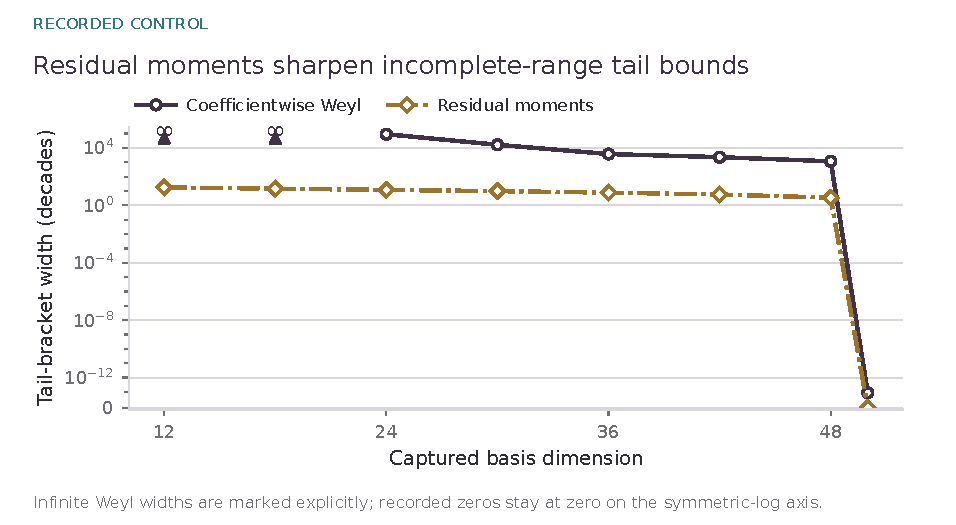
\includegraphics[width=\linewidth]{figures_production/figure_16_trace_moment_vs_weyl.pdf}
\caption{Range-dependent tail-bracket widths. The symmetric-log scale retains the recorded zero at full range capture. Residual moments preserve the amount and concentration of unresolved spectral mass, instead of assigning every coefficient the same worst-case radius. The first two Weyl widths are infinite and are explicitly marked by arrows rather than plotted as finite data.}
\label{fig:trace-moment-vs-weyl}
\end{figure}

A separate random implementation audit used 120 random factor/range pairs and
four admissible positive tilts per pair, for 480 MGF comparisons.  Both the
trace/cap and trace--Frobenius--cap envelopes dominated the exact log MGF in
every tested case.  The trace--Frobenius--cap form was at least as tight as the
trace/cap form in approximately 83.5\% of those comparisons.  This finite
sweep audits the implementation. The theorem above supplies the universal
argument.

\subsection{Residual rank from moments}

The same invariants determine when it is better to stop approximating the
missing spectrum and complete it exactly.  Let
\[
s=\operatorname{rank}F=\operatorname{rank}R.
\]
If the nonzero eigenvalues of \(R\) are \(r_1,\ldots,r_s\), then
\[
t=\sum_i r_i,
\qquad
v=\sum_i r_i^2,
\qquad
r_i\le\rho.
\]

\begin{theorem}[Residual-rank bracket]\label{claim:final-23-4}
\[
\boxed{
\left\lceil
\max\left\{
\frac{t}{\rho},
\frac{t^2}{v}
\right\}
\right\rceil
\le
\operatorname{rank}F
\le
n-r.
}
\]
The zero-residual case is interpreted separately as rank zero.
\end{theorem}

\begin{proof}
The inequality \(t\le s\rho\) gives \(s\ge t/\rho\).  Cauchy--Schwarz gives
\[
t^2
=
\left(\sum_{i=1}^s r_i\right)^2
\le
s\sum_{i=1}^s r_i^2
=sv,
\]
so \(s\ge t^2/v\).  Finally, every column of \(F\) lies in
\(\operatorname{range}(U)^\perp\), whose dimension is \(n-r\).
\end{proof}

Whenever the integer lower bound equals \(n-r\), the missing rank is certified
exactly without computing a residual SVD.

\begin{figure}[htbp]
\centering
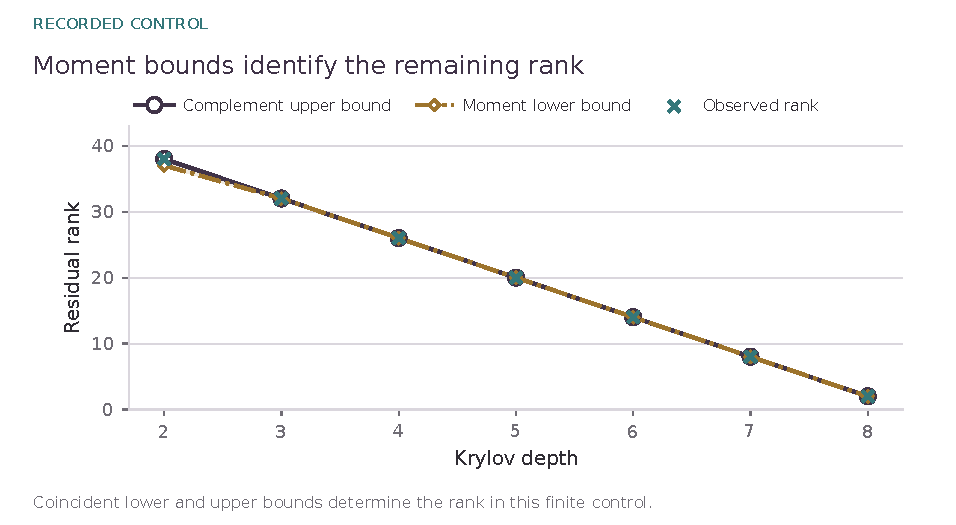
\includegraphics[width=\linewidth]{figures_production/figure_17_residual_rank_completion.pdf}
\caption{Moment lower bounds, complement upper bounds, and observed residual rank in the full-rank control. From depth three onward the bounds coincide. At depth eight only two residual directions remain, permitting a small exact completion.}
\label{fig:residual-rank-completion}
\end{figure}

\subsection{Exact residual completion}

Suppose a compact factorization of the residual is
\[
F=WD,
\]
where the columns of $W$ form an orthonormal basis of
$\operatorname{range}(F)$. Zero residual directions are omitted.
Since this range lies in the orthogonal complement of $U$,
\[
U^\top W=0.
\]

\begin{theorem}[Exact residual completion]\label{claim:final-23-5}
\[
\boxed{
A
=
[U\;W]
\begin{bmatrix}
B\\D
\end{bmatrix}.
}
\]
Consequently, the nonzero singular values of $A$ are exactly the nonzero
singular values, with multiplicity, of the stacked completion core
\[
\mathcal C_{\rm complete}
=
\begin{bmatrix}
B\\D
\end{bmatrix}.
\]
\end{theorem}

\begin{proof}
The decomposition $A=UB+F$ and the identity $F=WD$ give the factorization.
The matrix $[U\;W]$ has orthonormal columns, so
$A^\top A=\mathcal C_{\rm complete}^\top\mathcal C_{\rm complete}$.
The nonzero singular values therefore agree with multiplicity. If the
combined basis contains directions outside $\operatorname{range}(A)$,
its row Gram may include additional zeros. Its entire spectrum is the
nonzero spectrum of $AA^\top$ only when the combined basis spans exactly
$\operatorname{range}(A)$.
\end{proof}

This identity admits a column-streamed implementation.  For each residual
column block, project against the residual basis accumulated so far, append
only genuinely new directions through rank-revealing QR or SVD, and extend the
coordinate matrices of earlier blocks with zero rows.  New residual directions
are orthogonal to every earlier residual block by construction, so no earlier
data block must be revisited.

In the deterministic stress test, exact residual completion reproduced the
full singular spectrum at relative errors between approximately
\(2\times10^{-16}\) and \(6\times10^{-16}\) for all tested incomplete bases.
The resulting \(10^{-8}\) tail differed from the full-spectrum reference by
less than \(10^{-14}\) decades.  At depth 8 the candidate range had dimension
48, the missing rank was certified as exactly two, and appending those two
residual directions closed the spectrum without another approximate Krylov
stage.

\subsection{Hybrid stopping rule}

Residual information supplies a stopping rule for approximate iteration and
a handoff to exact completion:
\[
\boxed{
\begin{array}{c}
\text{streamed / pruned Krylov}\\[2mm]
\downarrow\\[-1mm]
\text{residual moments }(t,v,\rho)\\[2mm]
\downarrow\\[-1mm]
\begin{cases}
\text{continue Krylov}, & \text{residual range still large},\\
\text{exact streamed residual completion}, & \text{completion rank affordable}.
\end{cases}
\end{array}
}
\]

The trace-aware tail certificate remains useful as a rigorous intermediate
bound and as a stopping diagnostic.  Once only a small number of residual
directions remain, exact completion is mathematically preferable to forcing a
worst-case tail envelope to become artificially sharp.


\section{Verified matrix-to-spectrum bridge}\label{sec:final-6}

A tail enclosure is conditional on the spectrum supplied to it. To certify a
matrix-defined problem, the spectrum itself must be enclosed. This section
post-verifies a candidate eigensystem against the exact Gram matrix defined
by the stored factor entries. Chapter~\ref{ch:intervals} supplies the
positive-tail backend used at the endpoint of this construction.

\subsection{Binary64 input semantics}

Let
\[
A\in\mathbb R^{n\times m}
\]
be supplied as an IEEE binary64 array.  Each stored entry is treated as its
exact dyadic rational value.  The target operator is therefore the exact Gram
matrix
\[
H=AA^T
\]
defined by those binary64 values, not an unspecified nearby real matrix.

A high-precision symmetric eigensolver is used only to generate candidate
quantities
\[
Q\in\mathbb R^{n\times n},
\qquad
D=\operatorname{diag}(d_1,\ldots,d_n),
\qquad
d_1\ge\cdots\ge d_n\ge0.
\]
No correctness claim depends on trusting this eigensolver.

\subsection{Post-certified spectral enclosure theorem}

\begin{theorem}[Candidate eigensystem post-certification]\label{claim:final-6-1}
Let
\[
B=QDQ^T.
\]
Suppose directed-rounding computation proves
\[
\|Q^TQ-I\|_2\le\eta<1
\]
and
\[
\|H-B\|_2\le\rho.
\]
Then the ordered eigenvalues of the positive semidefinite matrix \(H\) satisfy
\[
\boxed{
\max\{0,(1-\eta)d_i-\rho\}
\le
\lambda_i(H)
\le
(1+\eta)d_i+\rho
}
\]
for every \(i\).
\end{theorem}

\begin{proof}
Set
\[
S=Q^TQ.
\]
The first hypothesis gives the Loewner inequalities
\[
(1-\eta)I\preceq S\preceq(1+\eta)I.
\]
The eigenvalues of
\[
B=(QD^{1/2})(QD^{1/2})^T
\]
are the same as those of
\[
D^{1/2}SD^{1/2}.
\]
Hence
\[
(1-\eta)D
\preceq
D^{1/2}SD^{1/2}
\preceq
(1+\eta)D,
\]
and eigenvalue monotonicity yields
\[
(1-\eta)d_i
\le
\lambda_i(B)
\le
(1+\eta)d_i.
\]
Weyl's perturbation inequality and
\(\|H-B\|_2\le\rho\) then give
\[
|\lambda_i(H)-\lambda_i(B)|\le\rho.
\]
Combining the two bounds and using \(H\succeq0\) proves the claim.
\end{proof}

The implementation does not attempt to evaluate the spectral norms above
exactly.  Instead it encloses every entry of
\[
Q^TQ-I
\quad\text{and}\quad
H-QDQ^T
\]
with directed-rounding interval arithmetic and uses
\[
\|M\|_2\le\|M\|_F.
\]
Thus the reported \(\eta\) and \(\rho\) are conservative certified upper
bounds.

\subsection{Monotone propagation into the tail}

Let the spectral theorem produce
\[
\ell_i\le\lambda_i(H)\le u_i.
\]
Using the same independent standard normals in all three sums gives
\[
\sum_i\ell_iZ_i^2
\le
\sum_i\lambda_iZ_i^2
\le
\sum_i u_iZ_i^2
\qquad\text{almost surely}.
\]
Therefore
\[
\boxed{
P\!\left(\sum_i\ell_iZ_i^2\ge q\right)
\le
P(Q\ge q)
\le
P\!\left(\sum_i u_iZ_i^2\ge q\right).
}
\]
The lower endpoint is evaluated by the rigorous positive-tail backend on the
lower spectrum, and the upper endpoint by the same backend on the upper
spectrum.  The controller requires more than two strictly positive
coefficients in each endpoint spectrum and a threshold above both endpoint
means.  An endpoint spectrum outside these implemented conditions is rejected
or reported as unsupported. Monotone coupling itself remains valid.  The final matrix-defined probability interval is accepted only when
its multiplicative ratio satisfies the requested accuracy.

\subsection{Random dense spectral-containment audit}

Three unrelated dense binary64 factors were tested against independently
recomputed high-precision eigenvalues of their exact dyadic Gram matrices:

\begin{center}
\begin{tabular}{@{}rrrr@{}}
\toprule
factor size & all eigenvalues contained & maximum relative width & time (s)\\
\midrule
$12\times18$ & yes & $3.36\times10^{-58}$ & 0.09\\
$20\times30$ & yes & $1.44\times10^{-57}$ & 0.35\\
$28\times36$ & yes & $1.20\times10^{-56}$ & 0.80\\
\bottomrule
\end{tabular}
\end{center}

No reference eigenvalue fell outside its certified interval.

\subsection{End-to-end matrix-defined tail near \texorpdfstring{\(10^{-16}\)}{1e-16}}

A dense \(64\times64\) exact-binary factor was constructed from a normalized
Hadamard basis with four singular-value groups.  The stored binary64 entries
are exact dyadic rationals.  The spectral postcheck returned
\[
\eta\le1.65\times10^{-49},
\qquad
\rho\le9.18\times10^{-50}.
\]
The leading coefficient, whose exact value is one in this control,
was enclosed with a width of order $10^{-49}$. The full outward-rounded
endpoints are preserved in the spectral record. Ellipsized decimal strings
are not used as interval endpoints.

At
\[
q=131.33201485100517,
\]
the tail lies near \(10^{-16}\).  Starting from the factor matrix itself:

\begin{center}
\begin{tabular}{@{}rrr@{}}
\toprule
requested relative accuracy & achieved ratio minus one & certified\\
\midrule
$10^{-10}$ & $2.60\times10^{-12}$ & yes\\
$10^{-12}$ & $4.09\times10^{-15}$ & yes\\
\bottomrule
\end{tabular}
\end{center}

For the \(10^{-12}\) request, the final enclosure was approximately
\[
\log_{10}p
\in
[-15.99999999999996625,
 -15.99999999999996447].
\]

This closes the basic numerical chain
\[
\boxed{
\text{binary64 factor}
\longrightarrow
\text{certified spectrum}
\longrightarrow
\text{certified deep-tail interval}
}
\]
at moderate matrix dimension.

\subsection{Scalability boundary}

The theorem applies in every finite dimension, but the present verifier forms a full candidate
basis \(Q\) and postchecks dense matrices.  It therefore closes the correctness
boundary before it closes the large-scale memory boundary.  For very large streamed factors, a memory-bounded guarantee would require a
verified range-core/residual certificate and an interval completion step in
place of the full-basis postcheck. Those extensions are not part of the
implemented dense verifier.



